\section{Common Control Platform (CCP)}
	
	\subsection{Hardware}
		\textbf{Indelprodukte}
		\begin{itemize}
			\item \textbf{COP-MAS2:} Das CPU-Board ist die zentrale Kontrolleinheit einer Indel Steuerung. Das CPU-Board koordiniert die Achsen und I/O-Systeme in Echtzeit. Alle Indel CPU-Boards werden mit dem Indel Echtzeitbetriebssystem INOS betrieben, dadurch ist es möglich, die gesamte Maschinenapplikation direkt auf dem CPU-Board zu implementieren. Das INOS Betriebssystem übernimmt die Abstraktion der gesamten Hardware und ermöglicht es damit, die gleiche Applikationssoftware auf beliebigen Indel CPU-Boards auszuführen.
			\item \textbf{SAC:} Endstufe zur Motoransteuerung mit integriertem Netzteil
			\item \textbf{SAM4:} High-End Alternative zum COP-MAS mit einer möglichen closed-loop frequenz bis $ 64kHz $.
		\end{itemize}
		\textbf{Besi-Produkte:}
		\begin{itemize}
			\item \textbf{Hammer S3 mit Connection-Board:} Äquivalente Endstufe zum SAC von ESEC selbstentwickelt.
			\item \textbf{UCB: } Notfalleinheit falls COP-MAS ausfällt übernimmt das UCB-Board die Steuerung
		\end{itemize}
		\begin{figure}[!h]
			\centering
			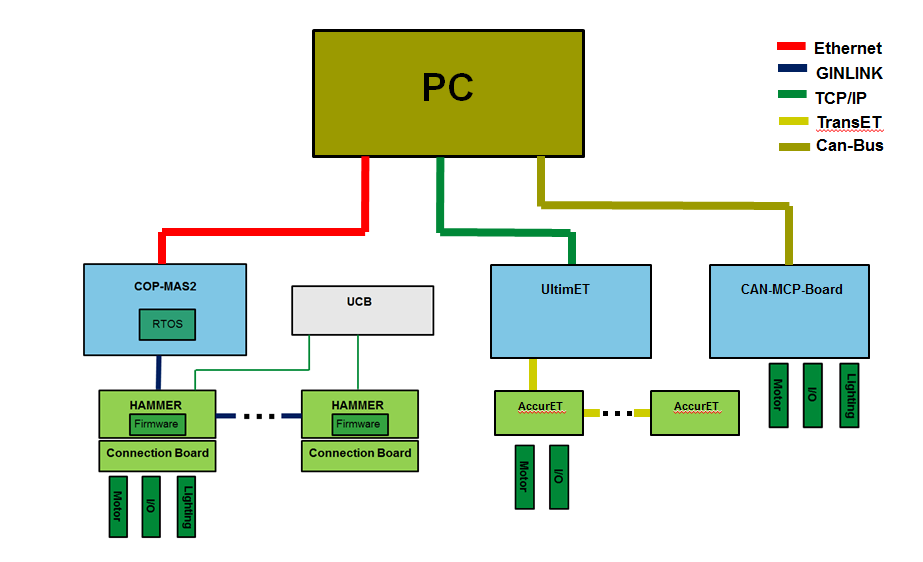
\includegraphics[width=0.85\linewidth]{./pics/ccp/mixed_struktur.png}
			\caption{Gemischte Struktur aus Indel und ETEL Controller}
		\end{figure}
	
		\subsubsection{Kompatibilität Hammer und Connection-Board}
			Beim Starten werden die ID`s der Hammer-Firmware und die ID des Connection-Boards (CB) verglichen. Die ID des CB's ist im Flashspeicher auf dem Board gespeichert. Das Board T128 benötigt dazu die Firmware N128 auf dem Hammer. 
			\begin{figure}[h!]
				\centering
				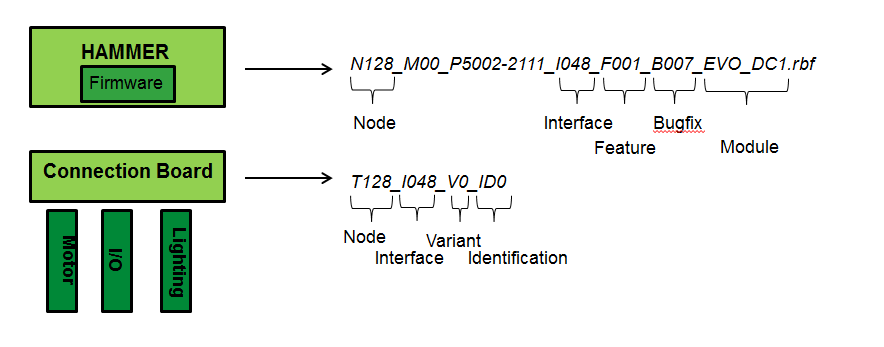
\includegraphics[width=0.8\linewidth]{./pics/ccp/connectionboard.png}
				\caption{ID Übereinstimmung}
			\end{figure}
			Die Identification und Variant kann über Dip-Switches am CB geändert werden. 
		
	\subsection{Konfiguration}
		Die Konfiguration eines Hammer-Boards geschieht anhand von zwei \textit{.dt2} Files, die auf dem MaschinenPC liegen.
		
		Im Source-Code ist der Pfad zu diesen Files hinterlegt. Diese \textit{.dt2} Files sind von Indel und werden direkt vom COP-MAS gelsen.
		\\\\
		Um den Konfigurationsaufwand zu erleichtern werden die Beiden \textit{.dt2} Files von Besi aus mehreren \textit{.dtx} Files erzeugt. Es wird also ein neues Front-End geschaffen, das handlicher zu ändern sein wird.
		



	